% IEEE Access submission. The official `ieeeaccess.cls` is not installed in the
% build environment used here; IEEEtran (the class ieeeaccess is derived from)
% is substituted so the manuscript compiles and paginates realistically.
% Swap the \documentclass line for ieeeaccess before submission.
\documentclass[journal]{IEEEtran}

\usepackage{amsmath,amssymb}
\usepackage{graphicx}
\usepackage[table]{xcolor}
\usepackage{booktabs}
\usepackage{array}
\usepackage{multirow}
\usepackage{cite}
\usepackage{url}

% ---- table palette (greyscale-safe: hues differ in luminance) --------------
\definecolor{hdr}{HTML}{1B3A6B}
\definecolor{hdralt}{HTML}{2C7F8F}
\definecolor{rowlite}{HTML}{EDF1F6}
\definecolor{okgreen}{HTML}{2F6B45}
\definecolor{warnred}{HTML}{8C2F39}
\definecolor{amberd}{HTML}{9A6912}
\definecolor{mist}{HTML}{DCE4EC}
\definecolor{pend}{HTML}{F5E7E4}

\newcommand{\hd}[1]{\textcolor{white}{\textbf{#1}}}
\newcommand{\yes}{\textcolor{okgreen}{\textbf{yes}}}
\newcommand{\no}{\textcolor{warnred}{\textbf{no}}}
\newcommand{\tbd}{\textcolor{warnred}{\textsc{pending}}}
\newcommand{\ns}{\textcolor{gray}{n/s}}

\begin{document}

\title{Characterizing the Laboratory-to-Field Gap and the On-Device
Feasibility Boundary for Crop Disease Diagnosis on ESP32-Class Hardware
with Closed-Loop Irrigation: A Baseline Audit and Pre-Registered
Evaluation Protocol}

\author{Author information withheld for review}

\markboth{IEEE Access}{Author information withheld for review}

\maketitle

\begin{abstract}
The pairing of a microcontroller sensing node, a camera module, a
convolutional leaf-disease classifier and a supervisory dashboard recurs
throughout the recent smart-agriculture literature, and building another
instance of it is not a research contribution. Three questions about that
architecture remain unresolved: how much of the accuracy such systems
report in the laboratory survives contact with field imagery captured by
their own camera; where the feasibility boundary for on-device inference
actually lies as a function of chip, quantization, class count and input
resolution; and whether closed-loop soil-moisture actuation reduces
delivered water against a metered fixed-schedule control on identical
hardware. This paper contributes an audited baseline and a pre-registered
protocol that answers them. The baseline classifier, a transfer-learned
YOLO11n-cls network fine-tuned on 43{,}444 laboratory-condition images
across 38 classes, reaches 99.32\,\% top-1 and 100\,\% top-5 validation
accuracy; we report this number as unaudited rather than as a result,
because the split that produced it is a naive per-class shuffle with no
duplicate-group awareness, and we quantify the leakage exposure that
follows. A static feasibility analysis of the exported artifact shows it
occupies 6.10\,MiB in FP32, some 12.0$\times$ the 520\,KiB on-chip SRAM of
the base ESP32, and that a single $224\times224\times3$ FP32 input
activation requires 588\,KiB, exceeding that budget before any intermediate
feature map is allocated; an ideal fourfold INT8 compression leaves the
artifact at 1.53\,MiB. From these bounds we pre-register falsifiable
predictions for the feasibility grid and the irrigation saving. Field
accuracy, on-device latency, power, per-node cost and flow-metered water
volume are identified as unmeasured and are reported as pending, not
estimated.
\end{abstract}

\begin{IEEEkeywords}
Precision agriculture, edge computing, TinyML, domain shift, dataset
leakage, closed-loop irrigation, ESP32, plant disease classification,
pre-registration.
\end{IEEEkeywords}

\section{Introduction}
\label{sec:intro}

\IEEEPARstart{P}{lant} disease is a first-order constraint on smallholder
yield, and the promise of automated diagnosis from leaf imagery has driven
a decade of applied deep-learning work in agriculture
\cite{mohanty2016deep,ferentinos2018deep,too2019comparative}. The
architecture that carries this promise into the field has converged: a
microcontroller-class board samples soil and environmental sensors, a
camera module supplies leaf images to a convolutional classifier, an
actuator closes an irrigation loop, and a cloud service exposes the result
to a grower. Instances of this architecture have been reported repeatedly,
with classification accuracies between 92\,\% and 98.6\,\%
\cite{samanta2024leafsense,nyakuri2025aiiot,aqasizade2026tinymlops}, and
the device-management substrate beneath it --- multi-tenant provisioning,
per-tenant data isolation, over-the-air update --- is a solved commercial
capability \cite{thingsboard,openremote}. Announcing another instance of
this architecture therefore contributes nothing, and this paper does not
attempt to.

What the published record leaves genuinely unresolved is narrower and more
consequential: whether the accuracy these systems report describes their
behaviour in the field at all.

\subsection{The Laboratory-to-Field Gap as the Framing Problem}

Most reported high-accuracy results in this literature are trained on the
PlantVillage corpus \cite{hughes2015plantvillage}, whose images are single
detached leaves photographed against uniform backgrounds under controlled
lighting. Mohanty~et~al.\ trained to 99.35\,\% held-out accuracy on that
corpus and then measured the same network on images drawn from outside it,
recording 31.4\,\% and 31.69\,\% \cite{mohanty2016deep}. The collapse was
reported by the original authors, not alleged by critics. It has since been
reproduced in form many times: Barbedo attributes it to the absence of
background clutter, lesion co-occurrence and capture variability in
laboratory corpora \cite{barbedo2018factors,barbedo2019plant}, and PlantDoc
was constructed specifically to provide a field-condition evaluation target
\cite{singh2020plantdoc}. On that target, the current cross-domain state of
the art for a PlantVillage-trained model is approximately 68\,\% top-1,
against 48\,\% for a ViT-Base backbone, 43\,\% for EfficientNet and 41\,\%
for InceptionV3 \cite{salman2025plantdisease}.

This is an instance of the general failure of i.i.d.\ evaluation under
distribution shift
\cite{torralba2011unbiased,recht2019imagenet,koh2021wilds}, compounded by
shortcut learning on backgrounds and acquisition artifacts
\cite{geirhos2020shortcut}. Its practical consequence for this literature
is specific: a headline accuracy above 95\,\% reported without a
cross-domain evaluation carries no information about deployed behaviour,
and is read by a reviewer as an unaudited number. A second, compounding
hazard is data leakage. Laboratory corpora contain near-duplicate frames of
the same physical leaf, and a split that is unaware of duplicate groups
places those near-duplicates on both sides of the partition, inflating
validation accuracy without any corresponding gain in generalization. This
mechanism is now recognised as a leading cause of irreproducible
machine-learning results across applied science \cite{kapoor2023leakage}.

\subsection{Cost and Connectivity Constraints of Smallholder Deployment}

A deployment intended for smallholders cannot assume reliable connectivity
or per-node budgets that support single-board computers with accelerators.
This pushes inference toward microcontroller-class silicon, where the TinyML
literature has established that useful models can run within a few hundred
kilobytes \cite{warden2019tinyml,david2021tflm,lin2020mcunet,lin2021mcunetv2}
under aggressive quantization \cite{jacob2018quantization,krishnamoorthi2018whitepaper},
and where standardised benchmarking is only beginning to mature
\cite{banbury2021mlperftiny}. The applied agricultural literature,
however, disagrees with itself about whether leaf-disease classification is
feasible on this class of hardware at all. Nyakuri~et~al.\ report that
ESP32-CAM, Raspberry Pi Pico and Arduino Nano 33 BLE Sense could not run
their model, and select a Raspberry Pi~5 instead --- 98.6\,\% accuracy,
16\,ms inference, \$80 per unit \cite{nyakuri2025aiiot}. Samanta~et~al.\
report a functioning ESP32-CAM deployment at 92\,\%
\cite{samanta2024leafsense}, and Aqasizade~et~al.\ report a quantized model
on ESP32-S3 at 94.6\,\% accuracy and 0.94 macro-F1 with a completed
seven-day field deployment \cite{aqasizade2026tinymlops}. No published work
resolves this disagreement along the axes that plausibly explain it: class
count, input resolution, quantization and chip variant.

\subsection{Research Questions and Hypotheses}
\label{sec:rqs}

\textbf{RQ1.} How much classification accuracy is lost when a model trained
on laboratory-condition imagery is evaluated on field imagery captured by
the system's own low-cost camera?

\emph{\textbf{H1.}} Accuracy falls substantially, with the residual sitting
near or below the $\approx$68\,\% cross-domain state of the art
\cite{salman2025plantdisease}. A field accuracy above 90\,\% is treated as
evidence of leakage or of an insufficiently varied field set, and is
investigated before being reported as a result.

\textbf{RQ2.} Where does the feasibility boundary for on-device inference
lie as a function of chip, quantization, class count and input resolution?

\emph{\textbf{H2.}} The base ESP32 fails above a threshold jointly set by
class count and input resolution; ESP32-S3 extends that boundary. The
specific predicted threshold is fixed in
Section~\ref{sec:prereg}, Table~\ref{tab:prereg}, and in
Figure~\ref{fig:predgrid}, before the sweep is executed.

\textbf{RQ3.} Does closed-loop soil-moisture actuation reduce delivered
water against a fixed schedule, and by how much under flow-meter
verification?

\emph{\textbf{H3.}} The reduction falls within the 9--50\,\% band reported
across the closed-loop irrigation literature, with a pre-registered point
prediction of $22\,\%\pm10\,\%$ (Section~\ref{sec:prereg}).

A hypothesis the data refutes is reported as refuted, in the body text,
not softened.

\subsection{Contributions}

\begin{enumerate}
\item \textbf{An audited baseline rather than a headline number.} We report
99.32\,\% top-1 laboratory accuracy and simultaneously demonstrate, from
the split procedure that produced it, why it cannot be treated as a
generalization estimate; we quantify the leakage exposure and specify the
duplicate-group-aware re-split that tests it (Section~\ref{sec:leakage}).

\item \textbf{A static feasibility analysis that bounds RQ2 before any
hardware sweep.} From measured artifact sizes and published memory budgets
we derive closed-form activation and storage bounds
(Equations~\ref{eq:act}--\ref{eq:compress}) showing that the binding
constraint at 224\,px is the input activation itself, not the weight
footprint, and we use those bounds to generate the pre-registered
feasibility grid (Section~\ref{sec:feas}).

\item \textbf{A resolution of the ESP32-class feasibility disagreement into
a measurable design space}, replacing the pass/fail claims in
\cite{nyakuri2025aiiot} and \cite{samanta2024leafsense} with a grid over
chip, precision, class count and resolution.

\item \textbf{A pre-registered, falsifiable evaluation protocol} for the
laboratory-to-field gap, the leakage audit, the feasibility sweep and a
flow-metered irrigation trial, with predictions and refutation criteria
fixed in advance (Section~\ref{sec:prereg}), following the registered-report
practice now established in the reproducibility literature
\cite{nosek2018preregistration,chambers2013registered,munafo2017manifesto}.

\item \textbf{An explicit negative disclosure.} We state which quantities
this work does not yet possess --- field accuracy, on-device latency,
power, per-node cost and metered water volume --- rather than substituting
estimates, and we show in Table~\ref{tab:related} that the resulting
comparison places this system behind published baselines on every axis
already measured.
\end{enumerate}

\section{Related Work}
\label{sec:related}

\subsection{IoT Sensing and Irrigation Platforms}

Automated irrigation driven by wireless soil sensing dates to
well-established work on GPRS-linked sensor networks
\cite{gutierrez2014automated}, and has since been extended with
machine-learning scheduling \cite{goap2018iot}, platform-scale water
management \cite{kamienski2019swamp}, and broad sensor-and-protocol surveys
\cite{garcia2020iot,vallejo2023smart}. Reported savings span roughly
9--50\,\%, a range wide enough that an unmetered claim within it is
uninformative. The methodological bar is set by trials that meter both
arms: Usman and Zubairu report 431.47\,L delivered under closed-loop
control against 592.39\,L under a fixed schedule --- a 27.16\,\% reduction
--- with soil-moisture standard deviations of 1.35\,\% and 10.46\,\%
respectively \cite{usman2026aiirrigation}, and Mohamed~et~al.\ report
improved water-use efficiency over a multi-season IoT deployment
\cite{mohamed2026iotirrigation}. Neither runs both arms on identical
low-cost microcontroller hardware and identical control software, which is
the comparison RQ3 isolates. Multi-tenant provisioning and per-tenant
isolation, often presented as system novelty, are commodity platform
features \cite{thingsboard,openremote} and are treated as such here.

\subsection{Deep Learning for Plant Disease Classification}

Following Mohanty~et~al.\ \cite{mohanty2016deep}, transfer learning from
ImageNet-pretrained backbones \cite{deng2009imagenet,he2016resnet,
szegedy2016inception} became the standard recipe, with reported accuracies
above 99\,\% on PlantVillage
\cite{ferentinos2018deep,too2019comparative,sladojevic2016deep,brahimi2017deep}.
Efficiency-oriented backbones \cite{howard2017mobilenets,sandler2018mobilenetv2,
tan2019efficientnet} and, more recently, vision transformers
\cite{dosovitskiy2021vit} have been substituted into the same recipe. The
classifier evaluated here is a YOLO11-family classification variant
\cite{ultralytics2024yolo11,redmon2016yolo}, chosen for its published
export path to embedded runtimes rather than for accuracy on this corpus.
Across this body of work the evaluation protocol, not the backbone, is the
limiting factor: Barbedo showed early that accuracy on laboratory imagery
is dominated by dataset properties rather than model capacity
\cite{barbedo2018factors}.

\subsection{Edge and TinyML Deployment on Constrained Hardware}

Microcontroller inference is bounded by SRAM for activations rather than by
flash for weights, a point made concrete by MCUNet's memory-aware
co-design \cite{lin2020mcunet} and its patch-based successor, which reduces
peak activation memory specifically to fit sub-megabyte parts
\cite{lin2021mcunetv2}. Deployment relies on post-training or
quantization-aware integer arithmetic \cite{jacob2018quantization,
krishnamoorthi2018whitepaper} executed by embedded interpreters such as
TensorFlow Lite for Microcontrollers \cite{david2021tflm,warden2019tinyml},
with MLPerf Tiny providing standard workloads \cite{banbury2021mlperftiny}.
Published engineering barriers on ESP32-class parts include interpreter
arena overflow, quantized-tensor misalignment, and contention between
inference, camera capture and the Wi-Fi stack within a few hundred
kilobytes of SRAM. Section~\ref{sec:feas} shows that for the artifact
studied here these barriers are predictable analytically, before any board
is flashed.

\subsection{The Laboratory-to-Field Domain Gap}

The gap is the central obstacle to deployment claims in this field. Its
canonical measurement remains Mohanty~et~al.'s own external evaluation
\cite{mohanty2016deep}; PlantDoc supplies a standard field-condition target
\cite{singh2020plantdoc}; and Salman~et~al.\ establish the current
cross-domain reference point at $\approx$68\,\%
\cite{salman2025plantdisease}. Table~\ref{tab:gap} collects this evidence.
Theoretical accounts of why the gap appears --- divergence between source
and target distributions \cite{bendavid2010theory}, dataset bias
\cite{torralba2011unbiased}, and reliance on spurious cues
\cite{geirhos2020shortcut} --- predict that the gap will be larger, not
smaller, when the target images come from a different optical path than
either training corpus. No published work measures the gap on imagery
captured by the deployed system's own camera, which differs from both
PlantVillage and PlantDoc in sensor, optics, compression and working
distance. That is the measurement RQ1 specifies.

\begin{table}[t]
\centering
\caption{Published laboratory-to-field accuracy evidence. Every value is
quoted from the cited source; the final row is this work's position, with
the field cell unmeasured rather than estimated.}
\label{tab:gap}
\footnotesize
\setlength{\tabcolsep}{4pt}
\begin{tabular}{p{2.45cm}ccc}
\rowcolor{hdr}
\hd{Study} & \hd{Lab} & \hd{Field / cross-dom.} & \hd{Drop} \\
\midrule
\rowcolor{rowlite}
Mohanty \cite{mohanty2016deep} & 99.35\,\% & 31.40\,\% & $-67.95$ \\
Mohanty \cite{mohanty2016deep} & 99.35\,\% & 31.69\,\% & $-67.66$ \\
\rowcolor{rowlite}
Salman, best \cite{salman2025plantdisease} & --- & 68.00\,\% & --- \\
Salman, ViT-B \cite{salman2025plantdisease} & --- & 48.00\,\% & --- \\
\rowcolor{rowlite}
Salman, EfficientNet \cite{salman2025plantdisease} & --- & 43.00\,\% & --- \\
Salman, InceptionV3 \cite{salman2025plantdisease} & --- & 41.00\,\% & --- \\
\rowcolor{pend}
\textbf{This work} & \textbf{99.32\,\%} & \tbd\ (E1) & \tbd \\
\bottomrule
\end{tabular}
\end{table}

\subsection{The Gap This Work Addresses}

No published study jointly (i) measures the accuracy lost when a
laboratory-trained classifier is evaluated on field images captured by its
own deployed camera rather than by a third-party field dataset, (ii)
reports the on-device feasibility boundary as a surface over class count,
resolution, precision and chip rather than as a single operating point, and
(iii) verifies an irrigation saving against a metered fixed-schedule
control on identical hardware and control software. Table~\ref{tab:related}
positions this work against the closest published systems. It is
constructed to include the columns on which this work is currently behind
--- field validation, measured latency, measured power --- rather than
omitting them.

\begin{table*}[t]
\centering
\caption{Comparison against published systems. Columns are chosen to
include the axes on which this work is currently \emph{weakest}; cells
marked \textsc{pending} are measurements identified in this paper's gap
analysis as not yet collected, and are not estimated. \ns\ = not stated in
the cited source.}
\label{tab:related}
\footnotesize
\setlength{\tabcolsep}{3.4pt}
\resizebox{\textwidth}{!}{%
\begin{tabular}{p{2.5cm}p{1.75cm}cccccccp{2.2cm}}
\rowcolor{hdr}
\hd{System} & \hd{Hardware} & \hd{Unit cost} & \hd{Inference} &
\hd{Accuracy} & \hd{Field-val.} & \hd{Latency} & \hd{Power} &
\hd{Closed-loop} & \hd{Dataset provenance} \\
\midrule
\rowcolor{rowlite}
Mohanty et al.\ \cite{mohanty2016deep} & offline & n/a & offline &
99.35\,\% / 31.4\,\% ext. & \no & n/a & n/a & \no &
100\,\% public (PlantVillage) \\
Salman et al.\ \cite{salman2025plantdisease} & offline & n/a & offline &
68\,\% cross-domain & \no & n/a & n/a & \no &
public (PlantVillage + PlantDoc) \\
\rowcolor{rowlite}
Nyakuri et al.\ \cite{nyakuri2025aiiot} & Raspberry Pi 5 & \$80 &
on-device & 98.6\,\% & \ns & 16\,ms & \ns & \no & \ns \\
Samanta et al.\ \cite{samanta2024leafsense} & ESP32-CAM & \ns & on-device &
92\,\% & \no & 850\,ms & \ns & \no & public benchmark \\
\rowcolor{rowlite}
Aqasizade et al.\ \cite{aqasizade2026tinymlops} & ESP32-S3 & \ns &
on-device & \textbf{94.6\,\% / 0.94 F1} & \textbf{\yes\ (7-day)} &
500\,ms & \ns & \no & public (PlantVillage-derived) \\
\rowcolor{pend}
\textbf{This work} & ESP32 + ESP32-CAM & \tbd & on-device (design) &
99.32\,\% lab, \emph{unaudited} & \no\ (E1 pending) & \tbd & \tbd &
\textbf{\yes} & \textbf{100\,\% public, 0 field-collected} \\
\bottomrule
\end{tabular}%
}
\end{table*}

Read honestly, Table~\ref{tab:related} shows this work behind
Aqasizade~et~al.\ \cite{aqasizade2026tinymlops} on field validation and on
every measured on-device quantity, and ahead only on closed-loop actuation,
which is an architectural property rather than a result. The contribution
claimed here is the audit and the protocol, not a superior system.

\section{Methodology}
\label{sec:methods}

\subsection{System Architecture}

The system comprises a field tier, a cloud tier and a client tier
(Figure~\ref{fig:arch}). A sensor and actuator node built on an ESP32
DevKit~V1 samples air temperature and relative humidity, soil moisture and
a rain indicator, and drives a single relay-switched pump. It transmits
telemetry every 10\,s and polls for operator commands every 5\,s over
HTTPS to a managed relational store. A physically separate ESP32-CAM node
performs demand-driven image capture, polling every 3\,s while idle and
streaming at no more than 4\,frames/s while a viewer is attached; it takes
no part in the irrigation decision. An application backend serves the
clients and runs a supervisory automation loop that may command the pump
under either a soil-moisture-threshold mode or a fixed-schedule timer mode;
the latter provides the control arm for the irrigation trial specified in
Section~\ref{sec:prereg}.

The property that matters for RQ3 is the locus of the control decision: the
irrigation rule of Equation~\ref{eq:pump} is evaluated on the node itself,
so actuation continues unchanged when the cloud tier is unreachable. Device
pairing and per-tenant isolation follow standard bearer-token and
row-level-isolation practice and are not treated further, being commodity
capability \cite{thingsboard,openremote}.

\begin{figure*}[t]
\centering
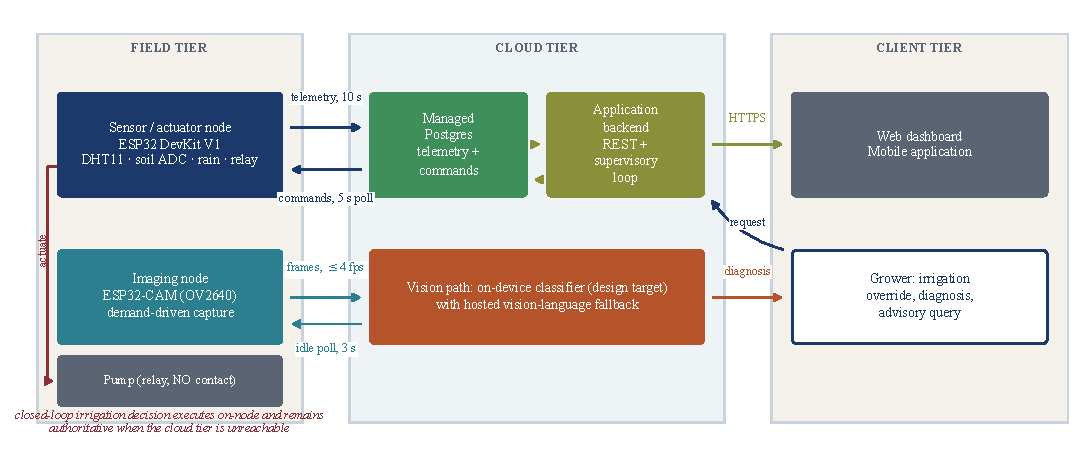
\includegraphics[width=\textwidth]{figures/fig_architecture.pdf}
\caption{Three-tier system organisation. Annotated periods and rate limits
are the deployed firmware constants. The irrigation decision is evaluated
on the sensing node, which is what allows the closed-loop arm of the
trial in Section~\ref{sec:prereg} to remain valid during connectivity
loss.}
\label{fig:arch}
\end{figure*}

\subsection{Hardware Design}

Figure~\ref{fig:hw} gives the sensing and actuation topology and
Table~\ref{tab:bom} its specifications. Three measurements are acquired
directly: air temperature and humidity from a DHT11 on a one-wire
interface, soil moisture from a capacitive probe on a 12-bit ADC channel,
and a binary rain indication from an active-low digital module. Two design
consequences are reported because they constrain what the system can
legitimately claim. First, root-zone temperature is not measured; it is
derived as a fixed $-2.5^{\circ}$C offset from air temperature, and is
therefore not an independent observation. Second, the camera bus on this
chip family occupies the same pins used for the soil ADC, the relay and the
sensor data line, which is why imaging runs on a second board rather than
on the sensing node --- a constraint with direct implications for RQ2,
since on-device inference must then share a part whose SRAM is already
committed to a frame buffer.

\begin{figure}[t]
\centering
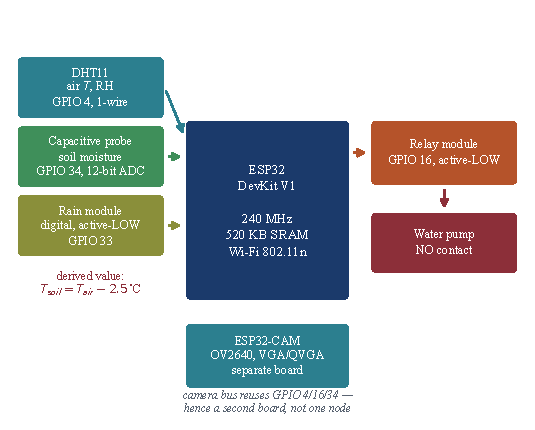
\includegraphics[width=\columnwidth]{figures/fig_hardware.pdf}
\caption{Sensing and actuation topology with pin assignments. Root-zone
temperature is a derived quantity, not a measured one.}
\label{fig:hw}
\end{figure}

\begin{table}[t]
\centering
\caption{Deployed sensing and actuation hardware. Per-unit costs are not
recorded in this project's records and are listed as pending rather than
estimated; the cost column is required before any cost claim appears in
this paper.}
\label{tab:bom}
\footnotesize
\setlength{\tabcolsep}{3pt}
\begin{tabular}{p{1.85cm}p{1.6cm}p{2.5cm}c}
\rowcolor{hdr}
\hd{Component} & \hd{Interface} & \hd{Specification} & \hd{Unit cost} \\
\midrule
\rowcolor{rowlite}
ESP32 DevKit V1 & --- & 240\,MHz dual-core, 520\,KiB SRAM, Wi-Fi 802.11n &
\tbd \\
ESP32-CAM & --- & AI-Thinker, OV2640, VGA/QVGA JPEG & \tbd \\
\rowcolor{rowlite}
DHT11 & 1-wire, GPIO 4 & air $T$, RH; 3 read attempts, 2.2\,s apart & \tbd \\
Capacitive probe & ADC, GPIO 34 & 12-bit; dry 4095, saturated 30 & \tbd \\
\rowcolor{rowlite}
Rain module & digital, GPIO 33 & active-low; no health check possible &
\tbd \\
Relay module & digital, GPIO 16 & active-low, normally-open contact & \tbd \\
\rowcolor{rowlite}
Pump & relay-switched & single actuation path & \tbd \\
Inline flow meter & --- & \emph{required for E4; not yet in the build} &
\tbd \\
\bottomrule
\end{tabular}
\end{table}

\subsection{Vision Model}

The classifier is a YOLO11n-cls network \cite{ultralytics2024yolo11}
initialised from pretrained weights and fine-tuned end to end at
$224\times224$ resolution over the 38-class species-and-condition taxonomy
of the PlantVillage corpus (Figure~\ref{fig:model}). The nano variant was
selected for its export path to embedded runtimes rather than for accuracy;
the feasibility analysis in Section~\ref{sec:feas} shows that even this
variant exceeds the target part's memory budget by an order of magnitude in
FP32, which is itself part of the RQ2 finding. A second-stage per-species
disease classifier and a four-corpus combined training configuration exist
in the pipeline but have not been executed; no result in this paper depends
on them.

\begin{figure*}[t]
\centering
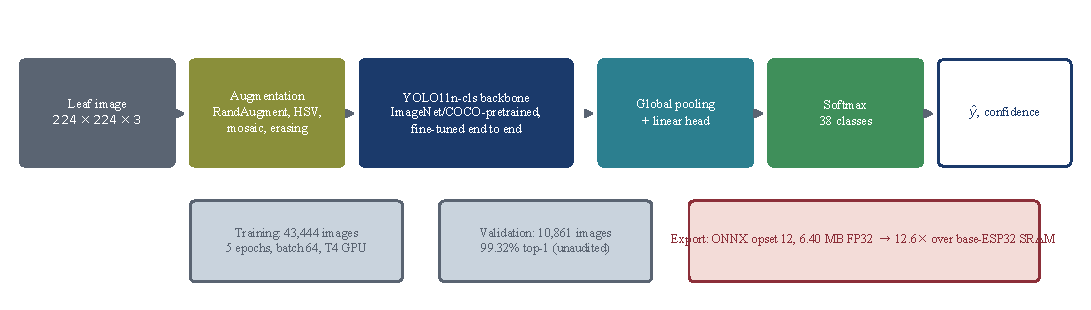
\includegraphics[width=\textwidth]{figures/fig_model.pdf}
\caption{Transfer-learning and export pipeline for the baseline classifier.
Values shown are the completed run's actual configuration and the measured
size of the exported artifact.}
\label{fig:model}
\end{figure*}

\subsection{Agronomic Reasoning Layer}

A reasoning component answers free-text agronomic queries grounded in live
telemetry and produces structured photo diagnoses when the on-device
classifier endpoint is unconfigured. The intended design places this
component behind a provider-agnostic adapter with an offline fallback so
that the reasoning backend is interchangeable without altering the client
contract. The implemented state does not yet match that design: the
component is bound to a single hosted provider, no adapter interface is
present, and no offline path exists, so the endpoint fails closed when the
provider is unreachable. This is reported as the current state rather than
the design goal, because the distinction determines what
``the deployed system's accuracy'' refers to: until the on-device serving
path is wired, application-level diagnoses do not originate from the
classifier this paper evaluates.

\subsection{Mathematical Formulation}

\subsubsection{Training objective}
The classifier minimises categorical cross-entropy over $C=38$ classes,
\begin{equation}
\mathcal{L}_{\mathrm{cls}} = -\frac{1}{N}\sum_{n=1}^{N}\sum_{i=1}^{C}
y_{n,i}\,\log \hat{y}_{n,i},
\label{eq:ce}
\end{equation}
with $y_n\in\{0,1\}^C$ the one-hot label, $\hat{y}_n$ the softmax output
and $N$ the batch size. Label smoothing is disabled, so $y$ is strictly
one-hot.

\subsubsection{Optimisation schedule}
The learning rate follows a linear warm-up over $E_w=3$ epochs and a cosine
decay \cite{loshchilov2017sgdr} from $\eta_0$ to $\eta_0\lambda_f$ over the
remaining epochs,
\begin{equation}
\eta(e)=
\begin{cases}
\eta_0\dfrac{e}{E_w}, & e \le E_w,\\[8pt]
\eta_0\!\left[\lambda_f+(1-\lambda_f)\dfrac{1+\cos\!\big(\pi\frac{e-E_w}{E-E_w}\big)}{2}\right],
& e > E_w,
\end{cases}
\label{eq:lr}
\end{equation}
with $\eta_0=0.01$, $\lambda_f=0.01$ and $E=5$.

\subsubsection{Evaluation metrics}
For a class with true positives $TP$, false positives $FP$, false negatives
$FN$ and true negatives $TN$,
\begin{align}
P &= \frac{TP}{TP+FP}, &
R &= \frac{TP}{TP+FN}, \label{eq:pr}\\
F_1 &= \frac{2PR}{P+R}, &
A &= \frac{TP+TN}{TP+TN+FP+FN}. \label{eq:f1}
\end{align}
Macro-averaging over classes,
\begin{equation}
F_1^{\mathrm{macro}} = \frac{1}{C}\sum_{i=1}^{C} F_{1,i},
\label{eq:macro}
\end{equation}
is reported alongside top-$k$ accuracy,
\begin{equation}
A_{@k} = \frac{1}{N}\sum_{n=1}^{N}
\mathbb{1}\!\left[y_n \in \mathrm{top}_k(\hat{y}_n)\right].
\label{eq:topk}
\end{equation}
Macro-averaging is required here rather than optional, because the
taxonomy is imbalanced by construction (Figure~\ref{fig:dataset}b).

\subsubsection{Domain gap}
The quantity RQ1 asks for is the signed difference between laboratory and
field accuracy on the same trained weights,
\begin{equation}
\Delta_{\mathrm{dom}} = A^{\mathrm{lab}}_{@1} - A^{\mathrm{field}}_{@1},
\label{eq:gap}
\end{equation}
reported together with both operands, never as a ratio, so that a small
$\Delta_{\mathrm{dom}}$ arising from a weak laboratory number cannot be
presented as robustness.

\subsubsection{Soil-moisture calibration}
A raw 12-bit reading $r$ is mapped to moisture percentage by a two-point
calibration against the deployed probe's dry-air and saturated-soil
readings $D=4095$ and $W=30$,
\begin{equation}
m(r) = \frac{D-r}{D-W}\times 100, \qquad r \ge r_{\mathrm{disc}},
\label{eq:soil}
\end{equation}
where readings below $r_{\mathrm{disc}}=10$ indicate a disconnected probe
and are rejected rather than converted, since an unplugged probe floats
near zero and would otherwise be indistinguishable from saturated soil.

\subsubsection{Irrigation decision rule}
Let $m_t$ be the calibrated moisture, $\rho_t\in\{0,1\}$ rain detection,
$s_t\in\{0,1\}$ probe health, $u_t\in\{-1,0,1\}$ the operator override and
$p_{t-1}$ the previous pump state. With hysteresis thresholds
$\theta_{\mathrm{dry}}=30$ and $\theta_{\mathrm{wet}}=70$,
\begin{equation}
p_t=
\begin{cases}
0, & s_t=0 \quad\text{(probe failed)}\\
0, & \rho_t=1 \quad\text{(rain)}\\
0, & m_t \ge \theta_{\mathrm{wet}}\\
0, & u_t=-1 \quad\text{(forced stop)}\\
1, & u_t=+1 \quad\text{(forced run)}\\
1, & m_t < \theta_{\mathrm{dry}}\\
p_{t-1}, & \text{otherwise (hold).}
\end{cases}
\label{eq:pump}
\end{equation}
The cases are evaluated in the order written (Figure~\ref{fig:irrig}), so
the three safety interlocks dominate operator intent: a manual run cannot
irrigate through rain, saturated soil or a failed probe. The trailing case implements the
anti-chatter hold band of Figure~\ref{fig:hyst}. Actuation is further
bounded by
\begin{equation}
\tau_{\mathrm{run}} \le 15\,\mathrm{min}, \qquad
\tau_{\mathrm{cool}} \ge 30\,\mathrm{min},
\label{eq:timers}
\end{equation}
a hard run cap and a subsequent cooldown that bound total delivery even
under a mis-calibrated probe. Equations~\ref{eq:pump} and \ref{eq:timers}
with the three constants stated reproduce the controller completely.

\begin{figure}[t]
\centering
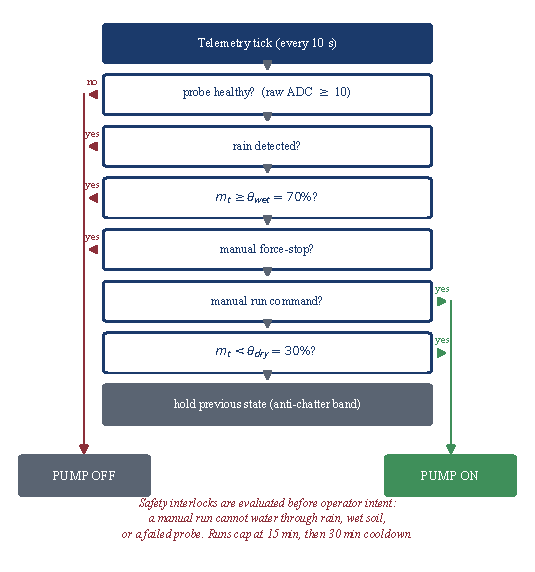
\includegraphics[width=\columnwidth]{figures/fig_irrigation.pdf}
\caption{Evaluation order of the irrigation rule of
Equation~\ref{eq:pump}. Safety interlocks precede operator intent by
construction.}
\label{fig:irrig}
\end{figure}

\begin{figure}[t]
\centering
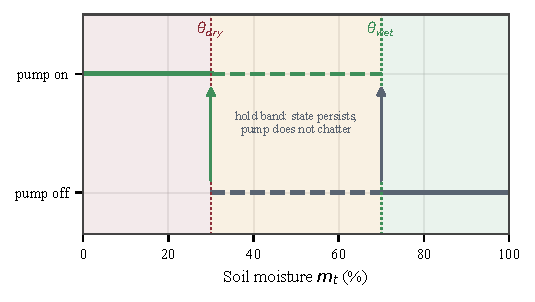
\includegraphics[width=\columnwidth]{figures/fig_hysteresis.pdf}
\caption{Hysteresis characteristic of the controller. Between
$\theta_{\mathrm{dry}}$ and $\theta_{\mathrm{wet}}$ the pump state
persists, which bounds actuation cycling; the width of this band is the
principal free parameter of the water-saving claim tested in RQ3.}
\label{fig:hyst}
\end{figure}

\subsubsection{Water-saving definition}
For the trial of Section~\ref{sec:prereg}, with $V_{\mathrm{cl}}$ and
$V_{\mathrm{fs}}$ the cumulative flow-metered volumes of the closed-loop
and fixed-schedule plots,
\begin{equation}
\Sigma = \frac{V_{\mathrm{fs}} - V_{\mathrm{cl}}}{V_{\mathrm{fs}}}\times 100,
\label{eq:saving}
\end{equation}
reported with both volumes and with the soil-moisture mean and standard
deviation of each plot, since a saving achieved by under-watering is not a
saving.

\subsubsection{Statistical comparison}
Model comparisons use the paired $t$-statistic over $s$ seeds,
\begin{equation}
t = \frac{\bar{d}}{\sigma_d/\sqrt{s}}, \qquad
\bar{d} = \frac{1}{s}\sum_{j=1}^{s} \big(a_j - b_j\big),
\label{eq:ttest}
\end{equation}
with $a_j,b_j$ the paired accuracies of two configurations under seed $j$,
at $\alpha=0.05$ \cite{demsar2006statistical}.

\subsubsection{On-device memory bounds}
The feasibility analysis of Section~\ref{sec:feas} rests on two bounds. The
input activation footprint for a square input of side $r$, $c$ channels and
$b$ bytes per element is
\begin{equation}
M_{\mathrm{act}}(r,c,b) = r^2\,c\,b,
\label{eq:act}
\end{equation}
which for the deployed configuration $r=224$, $c=3$ must satisfy
$M_{\mathrm{act}} + M_{\mathrm{inter}} + M_{\mathrm{fb}} + M_{\mathrm{sys}}
\le M_{\mathrm{SRAM}}$, where the remaining terms are intermediate feature
maps, the camera frame buffer and the system and network stack. The
weight-storage requirement induces a minimum compression ratio
\begin{equation}
\kappa_{\min} = \frac{S_{\mathrm{FP32}}}{S_{\mathrm{avail}}},
\label{eq:compress}
\end{equation}
with $S_{\mathrm{FP32}}$ the measured artifact size and
$S_{\mathrm{avail}}$ the addressable storage on the target part.

\subsubsection{Absence of a sensor--vision fusion rule}
Irrigation (Equation~\ref{eq:pump}) and diagnosis are independent decision
paths in the implemented system: neither consumes the other's output. No
numeric fusion rule exists, and none is presented; a fused decision rule is
identified as future work and appears in the ablation plan (E5) as a
configuration that must first be built.

\section{Results}
\label{sec:results}

\subsection{Dataset}
\label{sec:dataset}

Four corpora are configured in the data pipeline and one is reserved for
evaluation only (Table~\ref{tab:data}). Of these, only PlantVillage
\cite{hughes2015plantvillage} has been used in a completed training run;
the remaining three contribute zero images to every number in this paper.
This is stated plainly because a corpus that is configured is not a corpus
that is trained on, and the distinction is exactly the kind that inflates
dataset claims elsewhere in this literature.

\begin{table}[t]
\centering
\caption{Corpus manifest. Only the first row contributed to the completed
run. Licences are recorded only where the project's records state them;
unrecorded licences are marked rather than assumed.}
\label{tab:data}
\footnotesize
\setlength{\tabcolsep}{3pt}
\begin{tabular}{p{1.5cm}ccp{1.35cm}c}
\rowcolor{hdr}
\hd{Corpus} & \hd{Images} & \hd{Classes} & \hd{Licence} & \hd{Used} \\
\midrule
\rowcolor{rowlite}
PlantVillage & 54{,}305 & 38 & CC BY-SA 3.0 & \yes \\
PlantWild & 30{,}030 & 146 & CC BY-NC-ND 4.0 & \no \\
\rowcolor{rowlite}
Cassava & 21{,}367 & 5 & \ns & \no \\
Rice & 5{,}932 & 4 & \ns & \no \\
\rowcolor{mist}
\textbf{Sum of stated} & \textbf{111{,}634}\textsuperscript{$\dagger$} & --- &
--- & \textbf{54{,}305} \\
PlantDoc & \emph{eval only} & --- & \ns & \no\ (E1-c) \\
\bottomrule
\end{tabular}

\vspace{2pt}
\footnotesize
\textsuperscript{$\dagger$}Sum of the per-source counts stated in the
project's records. Those same records elsewhere give a training total of
``roughly 57{,}000'' images, which matches the three non-PlantVillage
sources alone. The discrepancy is unresolved pending a manifest build and
is recorded rather than silently reconciled; no result in this paper
depends on it, since only PlantVillage was used.
\end{table}

The completed run consumed 43{,}444 training and 10{,}861 validation
images, an 80/20 partition of 54{,}305 images over 38 classes. The taxonomy
is imbalanced by construction: tomato alone accounts for 10 of the 38
classes, while five crops contribute a single class each
(Figure~\ref{fig:dataset}b). This is the structural reason
Equation~\ref{eq:macro} rather than plain accuracy governs the per-class
reporting in E1 and E2.

\begin{figure*}[t]
\centering
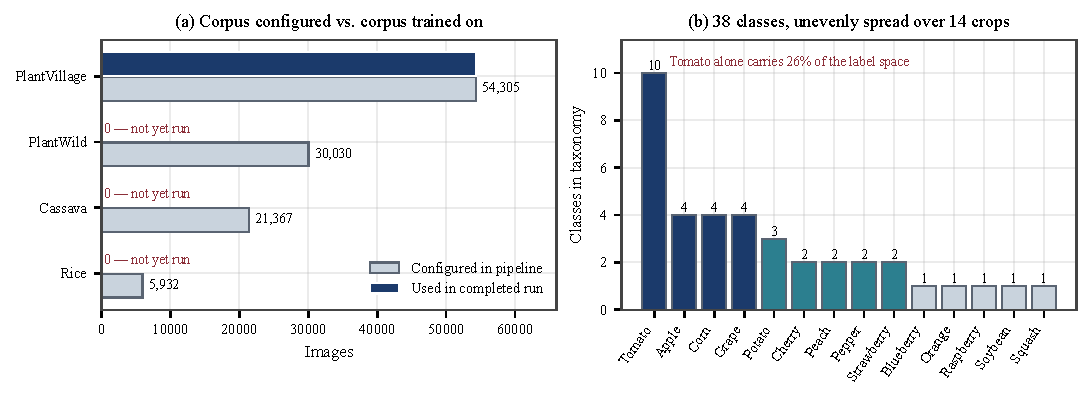
\includegraphics[width=\textwidth]{figures/fig_dataset.pdf}
\caption{(a) Corpus configured in the pipeline against corpus actually
consumed by the completed run; three of four configured sources contribute
nothing to any number reported here. (b) The 38-class taxonomy is
unevenly distributed over 14 crops, which is why macro-averaged metrics
are required.}
\label{fig:dataset}
\end{figure*}

All imagery is public and laboratory-conditioned; \emph{no field images
captured by this system's own camera exist}. Since that set is precisely
what RQ1 requires, its collection protocol is fixed here in advance: a
minimum of 300 images captured by the deployed camera node under variable
natural lighting, cluttered backgrounds, off-axis leaf presentation and
partial occlusion, hand-labelled against the same 38-class taxonomy, with
inter-annotator agreement reported for a duplicated subset.

Preprocessing and augmentation are applied in a fixed order: resize to
$224\times224$; RandAugment \cite{cubuk2020randaugment}; HSV jitter
($h{=}0.015$, $s{=}0.7$, $v{=}0.4$); translation 0.1 and scale 0.5;
horizontal flip $p{=}0.5$; mosaic $p{=}1.0$ \cite{bochkovskiy2020yolov4};
and random erasing $p{=}0.4$ \cite{zhong2020randomerasing}. Vertical flip,
rotation, shear, perspective, mixup, CutMix and copy-paste are disabled.
The augmentation policy matters for the leakage analysis below: mosaic and
erasing increase apparent sample diversity without adding independent
leaves, so they raise validation accuracy under a duplicate-unaware split
without necessarily improving generalization \cite{shorten2019survey}.

\subsection{Experimental Setup}

Table~\ref{tab:hyper} lists the complete configuration of the completed
run. Training used a single NVIDIA T4 GPU. All comparisons planned in E5
and E6 hold these settings fixed and vary only the factor under test, so
that the ablation isolates the intended variable. Target inference hardware
is the ESP32 DevKit~V1 and the AI-Thinker ESP32-CAM described in
Table~\ref{tab:bom}; an ESP32-S3 board required for the upper half of the
feasibility sweep has not yet been acquired, and the field site and trial
window for the irrigation experiment are not yet fixed.

\begin{table}[t]
\centering
\caption{Complete configuration of the completed training run. Identical
settings are held across every comparison planned in E5 and E6.}
\label{tab:hyper}
\footnotesize
\setlength{\tabcolsep}{3.5pt}
\begin{tabular}{p{1.95cm}p{1.65cm}p{1.8cm}p{1.05cm}}
\rowcolor{hdr}
\hd{Parameter} & \hd{Value} & \hd{Parameter} & \hd{Value} \\
\midrule
\rowcolor{rowlite}
Backbone & YOLO11n-cls & Pretrained & yes \\
Input resolution & $224\times224$ & Epochs & 5 \\
\rowcolor{rowlite}
Batch size & 64 & Seed & 42 \\
Optimiser & auto (SGD) & Deterministic & yes \\
\rowcolor{rowlite}
$\eta_0$ & 0.01 & $\lambda_f$ & 0.01 \\
Momentum & 0.937 & Weight decay & $5\times10^{-4}$ \\
\rowcolor{rowlite}
Warm-up epochs & 3 & Cosine LR & yes \\
Warm-up momentum & 0.8 & Warm-up bias LR & 0.1 \\
\rowcolor{rowlite}
Dropout & 0.0 & AMP & yes \\
Label smoothing & 0.0 & Nominal batch & 64 \\
\rowcolor{rowlite}
Auto-augment & RandAug. & Erasing & 0.4 \\
Mosaic & 1.0 & Mixup / CutMix & 0.0 / 0.0 \\
\rowcolor{rowlite}
HSV $h,s,v$ & 0.015, 0.7, 0.4 & Flip l/r, u/d & 0.5, 0.0 \\
Translate / scale & 0.1 / 0.5 & Rotation / shear & 0.0 / 0.0 \\
\bottomrule
\end{tabular}
\end{table}

\subsection{Experimental Results}

\subsubsection{Baseline convergence}
The run converges rapidly and monotonically (Figure~\ref{fig:curves},
Table~\ref{tab:epochs}). Validation loss falls from 0.210 to 0.024 and
top-1 validation accuracy rises from 94.75\,\% to 99.32\,\%, with top-5
saturating at 100\,\% by the third epoch. Total training cost was 21.7
minutes of single-GPU time.

\begin{table}[t]
\centering
\caption{Per-epoch results of the completed run, read directly from the
committed training log. Top-5 accuracy saturates at epoch 3, which is
itself a symptom discussed in Section~\ref{sec:leakage}.}
\label{tab:epochs}
\footnotesize
\setlength{\tabcolsep}{4.5pt}
\begin{tabular}{cccccc}
\rowcolor{hdr}
\hd{Epoch} & \hd{Train loss} & \hd{Val loss} & \hd{Top-1 (\%)} &
\hd{Top-5 (\%)} & \hd{Time (s)} \\
\midrule
\rowcolor{rowlite}
1 & 1.6892 & 0.2102 & 94.75 & 99.82 & 265.9 \\
2 & 0.1983 & 0.0712 & 97.87 & 99.97 & 524.7 \\
\rowcolor{rowlite}
3 & 0.1088 & 0.0383 & 98.91 & 100.00 & 780.5 \\
4 & 0.0745 & 0.0282 & 99.21 & 100.00 & 1040.4 \\
\rowcolor{rowlite}
\textbf{5} & \textbf{0.0524} & \textbf{0.0240} & \textbf{99.32} &
\textbf{100.00} & \textbf{1300.0} \\
\bottomrule
\end{tabular}
\end{table}

\begin{figure*}[t]
\centering
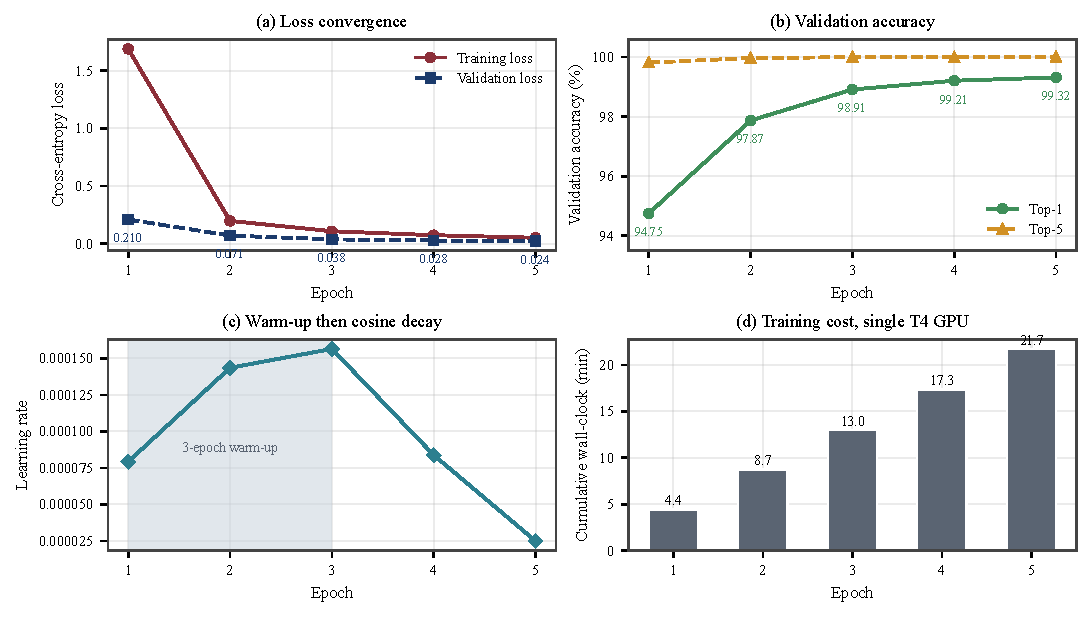
\includegraphics[width=\textwidth]{figures/fig_training_curves.pdf}
\caption{Baseline training dynamics, regenerated from the committed
training log. (a) Loss; (b) validation accuracy, with top-5 saturating at
epoch 3; (c) the warm-up-then-cosine schedule of Equation~\ref{eq:lr};
(d) cumulative wall-clock cost. No value is estimated.}
\label{fig:curves}
\end{figure*}

\begin{figure}[t]
\centering
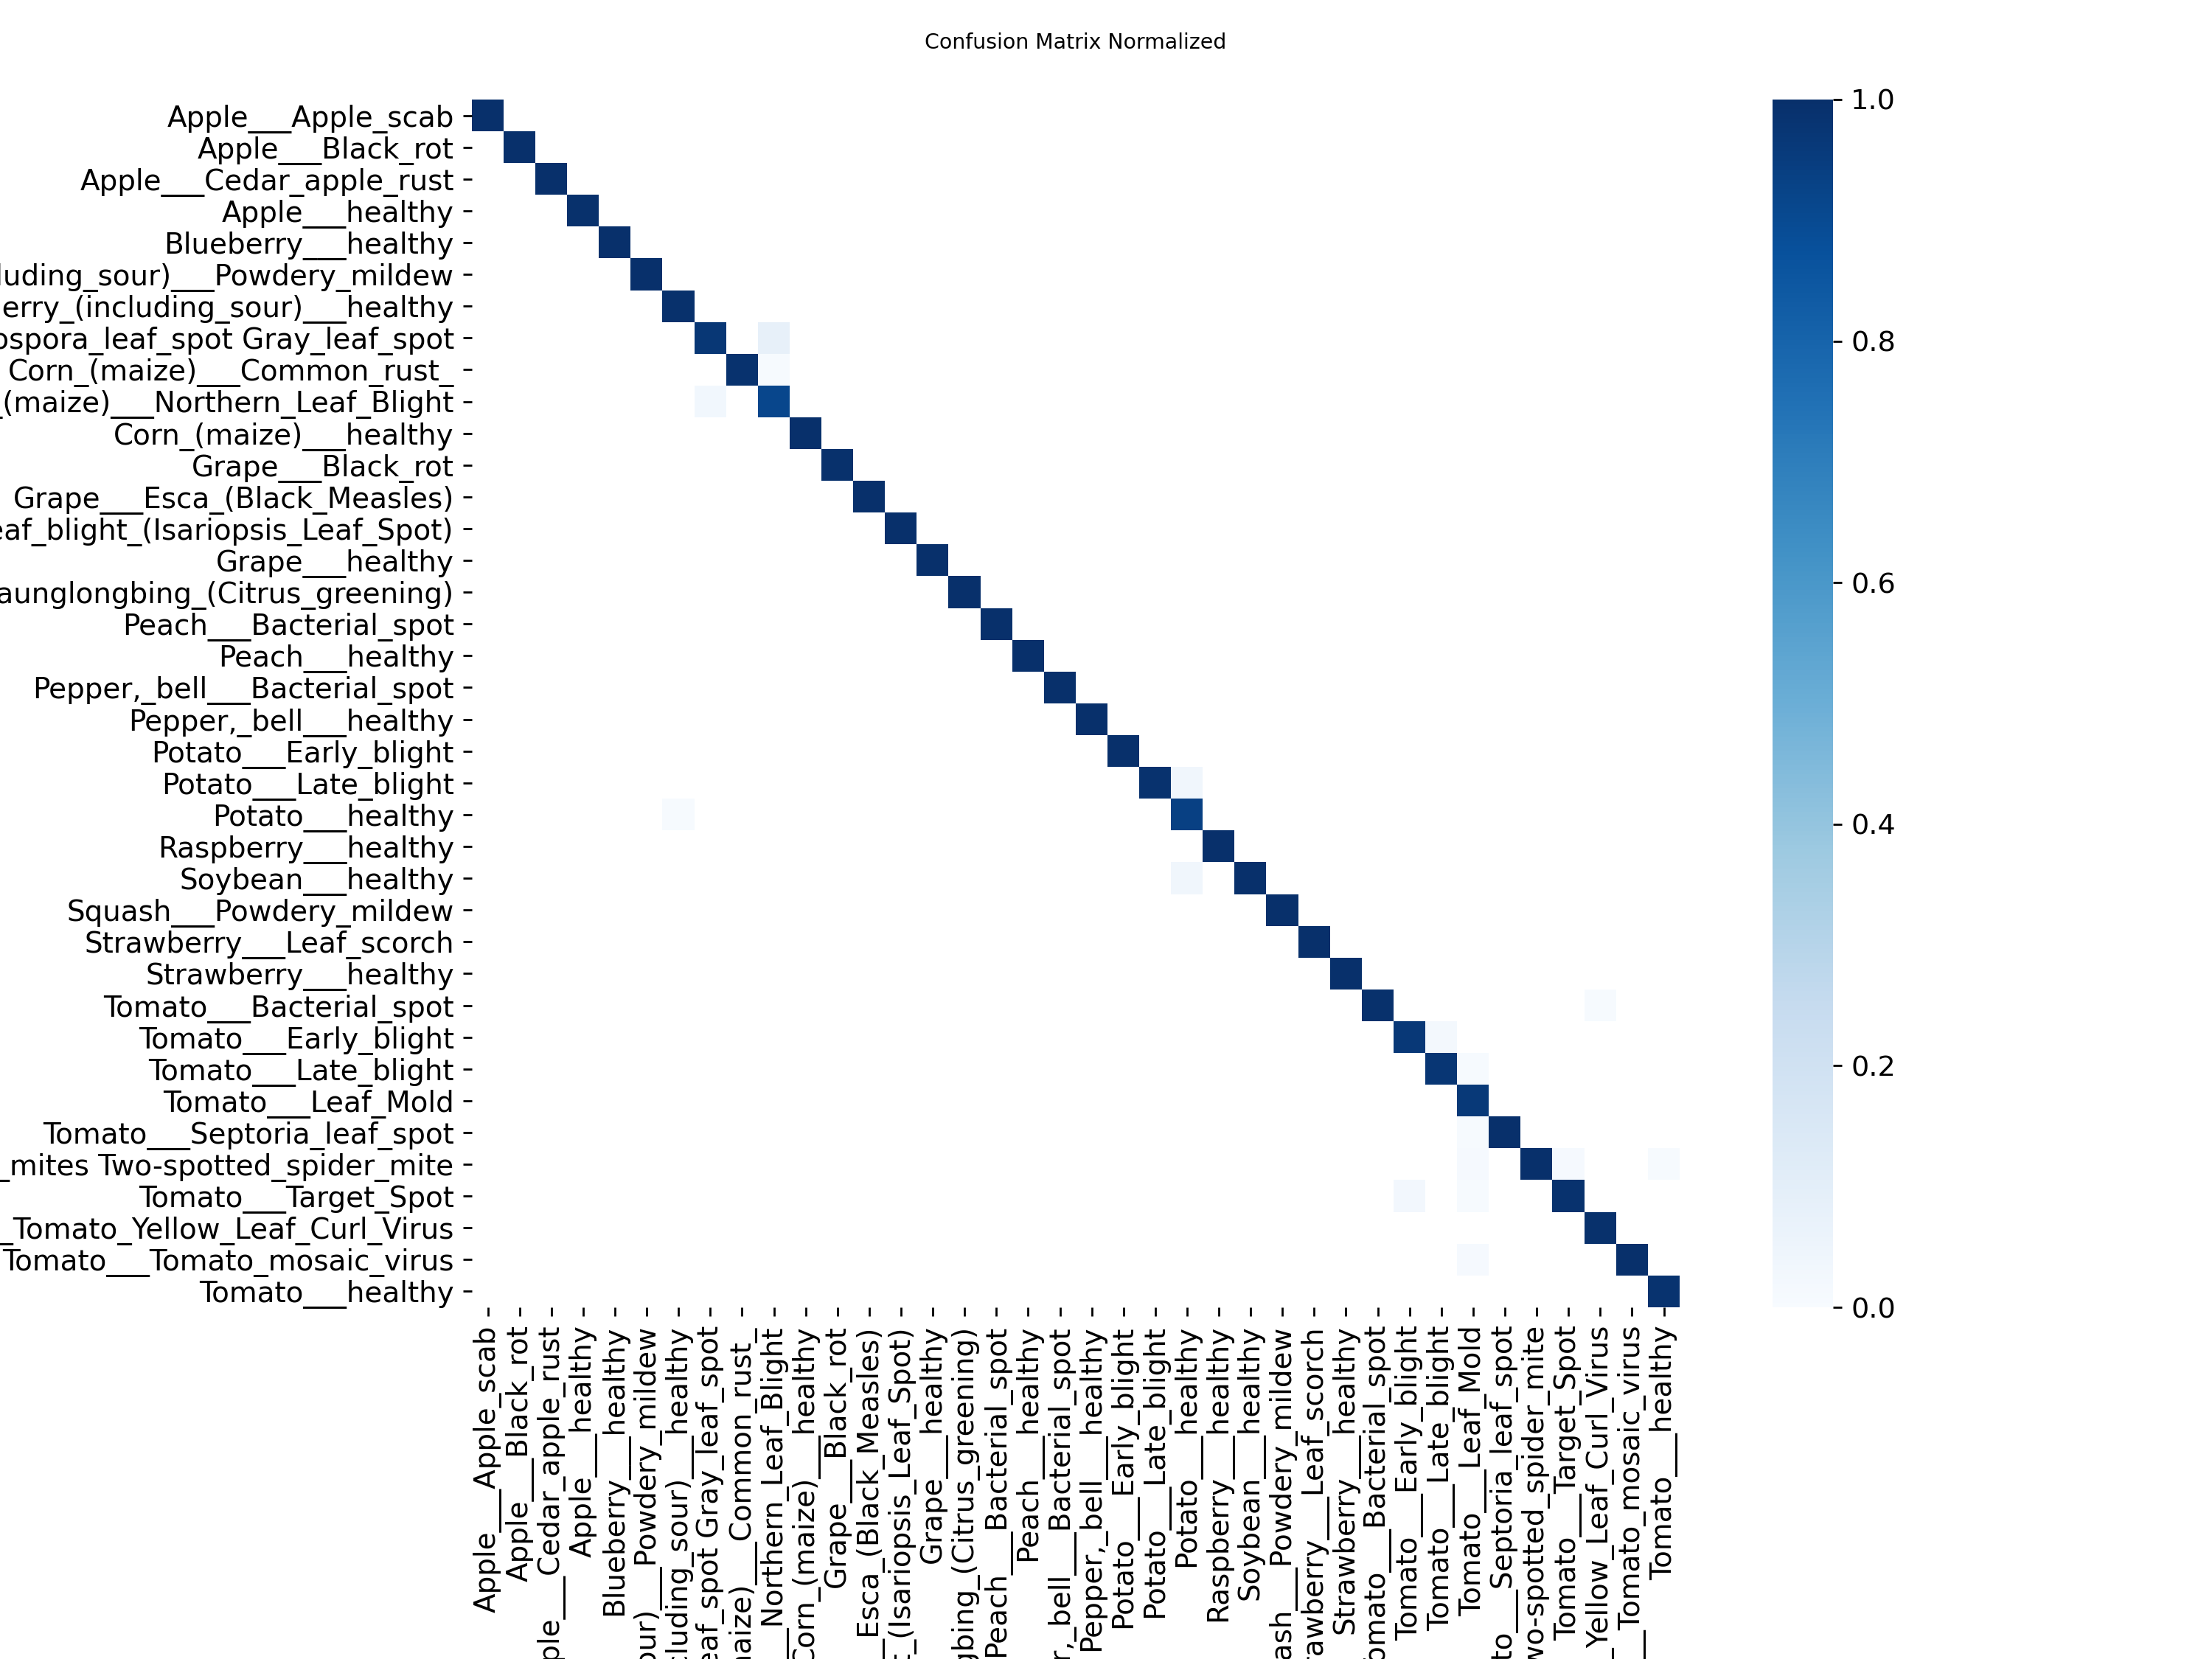
\includegraphics[width=\columnwidth]{figures/confusion_matrix_lab.png}
\caption{Normalised confusion matrix on the laboratory validation split,
produced by the completed run. The near-diagonal structure is what a
duplicate-unaware split predicts, and is not by itself evidence of
generalization; the field-condition counterpart (E1) does not yet exist.}
\label{fig:cmlab}
\end{figure}

The confusion matrix (Figure~\ref{fig:cmlab}) is almost perfectly diagonal.
We deliberately decline to present this as a strong result. A 38-class
problem solved to 99.32\,\% in five epochs from a pretrained backbone, with
top-5 saturating at 100\,\% by epoch three, is equally consistent with an
easy corpus, with leakage, or with both; distinguishing these requires E2,
not further discussion of the matrix.

\subsubsection{Leakage exposure of the reported baseline}
\label{sec:leakage}

The pipeline contains two distinct partitioning procedures, and the one
that produced the reported number is not the duplicate-aware one
(Table~\ref{tab:split}). The executed procedure shuffles each class
independently and slices an 80/20 partition, with no exact-duplicate
collapse, no perceptual-hash clustering and no notion of a duplicate group.
PlantVillage is known to contain multiple near-duplicate frames of the same
physical leaf; under this procedure nothing prevents one frame of such a
pair entering training and another entering validation.

\begin{table}[t]
\centering
\caption{The two partitioning procedures present in the pipeline. The
reported 99.32\,\% was produced by the left-hand column; the right-hand
column is implemented and unit-tested but has never been executed against
data.}
\label{tab:split}
\footnotesize
\setlength{\tabcolsep}{3pt}
\begin{tabular}{p{1.75cm}p{2.55cm}p{2.85cm}}
\rowcolor{hdr}
\hd{Property} & \hd{Executed (naive)} & \hd{Available (group-aware)} \\
\midrule
\rowcolor{rowlite}
Partition unit & individual image & duplicate group \\
Exact-duplicate collapse & none & SHA-256 \\
\rowcolor{rowlite}
Near-duplicate handling & none & perceptual hash, Hamming clustering \\
Cross-corpus overlap check & none & train/eval phash cross-check \\
\rowcolor{rowlite}
Stratification & per class & per (species, condition) \\
Ratios & 80/20 & 80/10/10 \\
\rowcolor{rowlite}
Verified by tests & --- & 4 unit tests, passing \\
\rowcolor{pend}
\textbf{Status} & \textbf{produced 99.32\,\%} & \textbf{never run (E2)} \\
\bottomrule
\end{tabular}
\end{table}

We therefore report the exposure rather than an inflation estimate: the
magnitude of any inflation is unknown until the group-aware re-split is
executed and the model retrained under identical settings, which is E2.
Reporting an estimated correction here would substitute an assumption for a
measurement, which is the failure mode this paper is organised against
\cite{kapoor2023leakage}. The direction, however, is predictable: under a
group-aware split, accuracy can only fall or remain equal, never rise.

\subsubsection{Static feasibility analysis}
\label{sec:feas}

RQ2 can be partially bounded without flashing a board, and the bound is
informative. The exported FP32 artifact measures 6{,}396{,}724\,bytes
(6.10\,MiB) and the training checkpoint 3{,}279{,}554\,bytes (3.13\,MiB).
Against the 520\,KiB of on-chip SRAM on the base ESP32, the exported
artifact is $12.0\times$ oversized by Equation~\ref{eq:compress}; an ideal
fourfold INT8 compression \cite{jacob2018quantization} leaves 1.53\,MiB,
still $3.0\times$ the SRAM budget, although within typical module flash
(Figure~\ref{fig:mem}).

\begin{figure}[t]
\centering
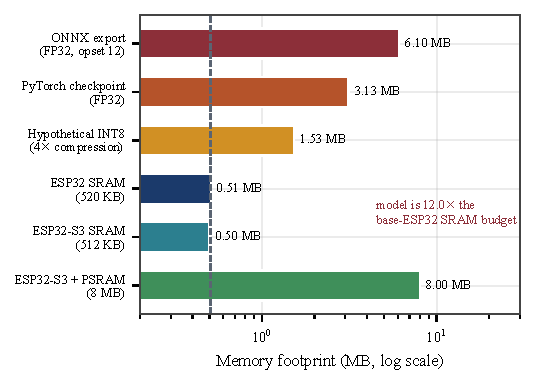
\includegraphics[width=\columnwidth]{figures/fig_memory.pdf}
\caption{Measured artifact footprints against published on-chip memory
budgets, log scale. The FP32 export exceeds base-ESP32 SRAM by
$12.0\times$; even an ideal INT8 quantization remains $3.0\times$ over.}
\label{fig:mem}
\end{figure}

The sharper constraint is activation memory, and it is the reason the
resolution axis dominates the feasibility surface. Applying
Equation~\ref{eq:act} to the input tensor alone, before any intermediate
feature map is allocated, gives Table~\ref{tab:actmem}: at $224\times224$
in FP32 the input activation alone requires 588\,KiB and therefore cannot
be resident in a 520\,KiB SRAM under any interpreter, whereas the same
tensor in INT8 requires 147\,KiB and the $96\times96$ INT8 case requires
27\,KiB. This analysis reconciles the apparent contradiction in the
literature: the ESP32-CAM failure reported by Nyakuri~et~al.\
\cite{nyakuri2025aiiot} and the successful ESP32-S3 deployment of
Aqasizade~et~al.\ \cite{aqasizade2026tinymlops} are not in conflict once
resolution and precision are treated as free variables rather than fixed
implementation details, which is exactly the claim H2 formalises. It also
explains why patch-based execution is the standard remedy at this scale
\cite{lin2021mcunetv2}.

\begin{table}[t]
\centering
\caption{Input-activation footprint from Equation~\ref{eq:act}, for the
input tensor alone. Cells exceeding the 520\,KiB base-ESP32 SRAM budget
are infeasible before any intermediate feature map, frame buffer or network
stack is accounted for.}
\label{tab:actmem}
\footnotesize
\setlength{\tabcolsep}{4pt}
\begin{tabular}{ccccc}
\rowcolor{hdr}
\hd{Resolution} & \hd{Elements} & \hd{INT8} & \hd{FP32} &
\hd{FP32 vs SRAM} \\
\midrule
\rowcolor{rowlite}
$96\times96\times3$ & 27{,}648 & 27\,KiB & 108\,KiB & 21\,\% \\
$128\times128\times3$ & 49{,}152 & 48\,KiB & 192\,KiB & 37\,\% \\
\rowcolor{pend}
$224\times224\times3$ & 150{,}528 & 147\,KiB & \textbf{588\,KiB} &
\textcolor{warnred}{\textbf{113\,\% --- infeasible}} \\
\bottomrule
\end{tabular}
\end{table}

A further term is specific to this system. Because the camera bus and the
sensing pins collide on one part (Section~\ref{sec:methods}), imaging and
inference must share a board whose SRAM already holds a frame buffer: a
QVGA RGB565 buffer alone occupies 150\,KiB, or 29\,\% of the base part's
SRAM, before any model tensor is allocated. The hardware partitioning
decision and the feasibility boundary are thus the same question, which is
not visible when feasibility is reported as a single pass/fail figure.

\subsubsection{Quantities not yet measured}

Field accuracy, per-class field precision and recall, on-device latency,
peak RAM in situ, energy per inference, end-to-end sensor-to-decision
latency, uptime, packet loss, per-node cost and flow-metered water volume
do not exist for this system. They are listed with their measurement
procedures in Table~\ref{tab:prereg} and are not estimated anywhere in this
paper, including in the abstract.

\subsection{Pre-Registered Protocol and Predictions}
\label{sec:prereg}

The experiments that answer RQ1--RQ3 are specified here in advance, with
predictions and refutation criteria fixed before execution
(Figure~\ref{fig:protocol}, Table~\ref{tab:prereg}). Pre-registration is
adopted because the principal threat to this paper's central claim is the
temptation to reinterpret a disappointing field number after seeing it
\cite{nosek2018preregistration,chambers2013registered}.

\begin{figure*}[t]
\centering
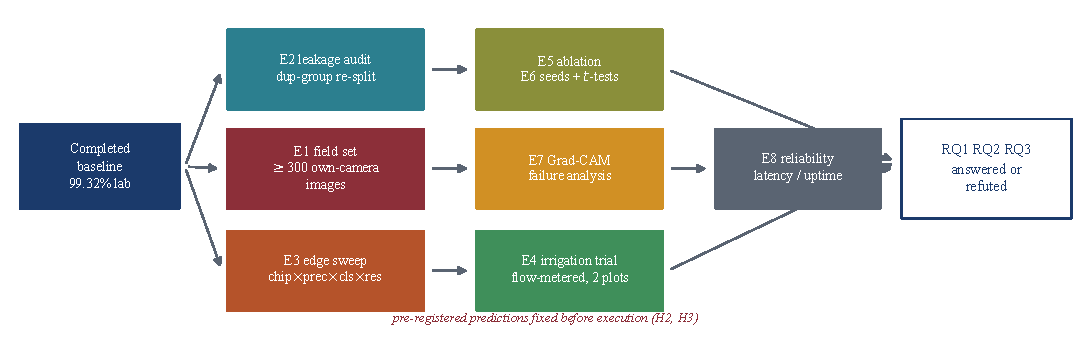
\includegraphics[width=\textwidth]{figures/fig_protocol.pdf}
\caption{Dependency structure of the pre-registered protocol. E1 gates the
domain-gap and explainability results; E2 gates every accuracy claim; E3
and E4 are independent of both.}
\label{fig:protocol}
\end{figure*}

\begin{table*}[t]
\centering
\caption{Pre-registered experimental protocol. Predictions and refutation
criteria are fixed before execution; no cell of this table is a
measurement.}
\label{tab:prereg}
\footnotesize
\setlength{\tabcolsep}{4pt}
\begin{tabular}{p{0.5cm}p{3.5cm}p{4.6cm}p{3.5cm}p{3.3cm}}
\rowcolor{hdr}
\hd{ID} & \hd{Quantity} & \hd{Procedure} & \hd{Pre-registered prediction} &
\hd{Refutation criterion} \\
\midrule
\rowcolor{rowlite}
E1 & Field top-1 and macro-F1 on own-camera imagery &
$\ge$300 hand-labelled images from the deployed camera node under varied
lighting, clutter, off-axis pose, occlusion; evaluate unchanged weights &
$A^{\mathrm{field}}_{@1} \le 68\,\%$; $\Delta_{\mathrm{dom}} \ge 30$ points &
$A^{\mathrm{field}}_{@1} > 90\,\%$ implies leakage or an insufficiently
varied field set; investigate before reporting \\
E2 & Leakage delta &
Duplicate-group-aware re-split, identical retraining settings, compare with
99.32\,\% &
Accuracy falls; group-aware top-1 $<$ 99.32\,\% &
No fall indicates the corpus lacks exploitable near-duplicates; report as
such \\
\rowcolor{rowlite}
E3 & Feasibility grid: fits, accuracy, size, latency, peak RAM, energy &
Chip $\times$ precision $\times$ class count $\times$ resolution, flashed
and measured on hardware &
Base ESP32 fails at 224\,px FP32 for all class counts
(Equation~\ref{eq:act}); fails at 16 classes / 224\,px in both precisions;
ESP32-S3 fits 16 classes / 224\,px INT8 &
Base ESP32 fitting at 224\,px FP32, or ESP32-S3 failing at 8 classes /
128\,px, refutes H2 as stated \\
E4 & Water volume, soil-moisture mean and SD, plant-health proxy &
Two plots, inline flow meter, closed-loop vs fixed-schedule, $\ge$2 weeks,
identical hardware and control software &
$\Sigma = 22\,\% \pm 10\,\%$ (interval 12--32\,\%), below the 27.16\,\%
of \cite{usman2026aiirrigation} because that controller is strictly more
expressive than Equation~\ref{eq:pump} &
$\Sigma \notin [12,32]\,\%$, including $\Sigma \le 0$, refutes H3 \\
\rowcolor{rowlite}
E5 & Ablation &
Backbone alone; $+$augmentation; FP32 vs INT8; sensor-only vs vision-only
vs fused, identical settings &
Augmentation contributes $<$1 point under a group-aware split &
--- \\
E6 & Significance &
$\ge$4 seeds, mean$\pm$SD, paired $t$-tests (Equation~\ref{eq:ttest}),
$\alpha=0.05$ &
--- & --- \\
\rowcolor{rowlite}
E7 & Explainability &
Grad-CAM \cite{selvaraju2017gradcam} on correct and incorrect predictions
per class, including $\ge$1 field failure &
Field failures attend to background rather than lesion
\cite{geirhos2020shortcut} &
Lesion-centred attention on field failures refutes the shortcut
explanation \\
E8 & Reliability &
Sensor-to-decision latency distribution, uptime, packet loss over the trial
window & --- & --- \\
\bottomrule
\end{tabular}
\end{table*}

\begin{figure}[t]
\centering
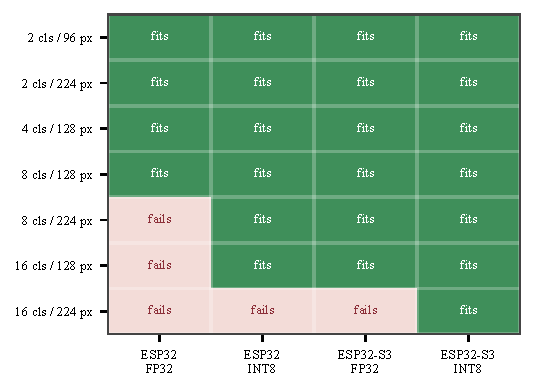
\includegraphics[width=\columnwidth]{figures/fig_prediction_grid.pdf}
\caption{Pre-registered H2 feasibility prediction, derived from
Equations~\ref{eq:act} and \ref{eq:compress}. \emph{This figure contains no
measurements}; it is the falsifiable prediction against which the E3 sweep
will be scored.}
\label{fig:predgrid}
\end{figure}

\subsection{Discussion}
\label{sec:discussion}

\subsubsection{RQ1 --- the laboratory-to-field gap}
RQ1 is not yet answered, and this paper does not answer it by proxy. What
it establishes is the bound within which the answer must fall and the
criterion by which it will be judged. The published evidence
(Table~\ref{tab:gap}, Figure~\ref{fig:gap}) places comparable
PlantVillage-trained models between 31\,\% and 68\,\% on field-condition
imagery. Our laboratory operand, 99.32\,\%, sits at the top of the
published laboratory range, which under H1 implies a large
$\Delta_{\mathrm{dom}}$ rather than a favourable one: a model that has
partially memorised near-duplicates has less, not more, to transfer. The
single most likely outcome, stated in advance, is a field accuracy in the
40--68\,\% band and $\Delta_{\mathrm{dom}}$ of 30--60 points.

\begin{figure}[t]
\centering
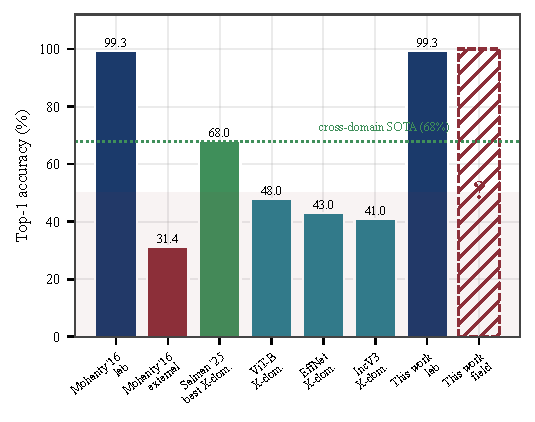
\includegraphics[width=\columnwidth]{figures/fig_gap.pdf}
\caption{Published laboratory and cross-domain accuracies with this work's
position. The hatched bar is the unmeasured quantity RQ1 targets; the
dotted line is the cross-domain state of the art against which H1 is
scored.}
\label{fig:gap}
\end{figure}

\subsubsection{RQ2 --- the feasibility boundary}
RQ2 is partially answered analytically and not yet answered empirically.
The contribution of Section~\ref{sec:feas} is to show that the
disagreement in the literature is resolvable in principle: once resolution
and precision are treated as free variables, the Raspberry-Pi-5 selection
of \cite{nyakuri2025aiiot} and the successful ESP32-S3 deployment of
\cite{aqasizade2026tinymlops} describe different points on one surface
rather than contradictory facts about a chip. Equation~\ref{eq:act} shows
the binding constraint at 224\,px is the input activation, not the weight
footprint --- a distinction that matters because the standard remedy for
oversized weights, quantization, does not by itself relieve an activation
bound, whereas reducing resolution does, quadratically. The empirical grid
that would confirm this is E3.

\subsubsection{RQ3 --- closed-loop water saving}
RQ3 is not yet answered, and by the rule stated in
Section~\ref{sec:intro} no water-saving figure appears anywhere in this
paper, including the abstract. The pre-registered prediction of
$22\,\%\pm10\,\%$ is reasoned downward from the 27.16\,\% of
\cite{usman2026aiirrigation}: that trial's controller schedules irrigation
from a learned regression model, a strictly more expressive control law
than the two-threshold hysteresis of Equation~\ref{eq:pump}, so an equal or
larger saving from a simpler controller would be surprising. The interval
is widened because the planned trial is single-site and single-season.

\subsubsection{Threats to validity}
Four threats dominate. \emph{Construct validity:} the laboratory number
measures performance on detached leaves against uniform backgrounds, which
is not the construct of interest. \emph{Internal validity:} the executed
split permits near-duplicate leakage (Section~\ref{sec:leakage}), so the
baseline is an upper bound on the true laboratory generalization, not an
estimate of it. \emph{External validity:} a single site, a single season
and a 38-class taxonomy dominated by one crop bound what any field result
can generalise to. \emph{Statistical validity:} the reported baseline is a
single seed; no variance estimate exists until E6 supplies one, and single-
seed differences of a fraction of a point are not interpretable
\cite{demsar2006statistical}.

\subsubsection{What would falsify the paper's own framing}
If E2 returns no accuracy drop under a group-aware split and E1 returns
field accuracy above 90\,\%, then the framing adopted here --- that
laboratory numbers in this literature are systematically optimistic --- is
wrong for this corpus and system, and the paper would report that. The
framing is offered as a testable position, not an assumption.

\section{Conclusion}
\label{sec:conclusion}

This paper contributes an audited baseline, a static feasibility analysis
and a pre-registered protocol for on-device crop disease diagnosis with
closed-loop irrigation on ESP32-class hardware. The baseline classifier
attains 99.32\,\% top-1 and 100\,\% top-5 accuracy on laboratory-condition
validation data, and we report that number together with the reason it
cannot yet be read as a generalization estimate: the split that produced
it is duplicate-unaware, and the group-aware re-split that would test the
exposure has not been run. The feasibility analysis establishes, from
measured artifact sizes and published memory budgets, that the exported
FP32 model exceeds base-ESP32 SRAM by $12.0\times$, that an ideal INT8
quantization leaves it $3.0\times$ oversized, and that at $224\times224$
the input activation alone requires 588\,KiB against a 520\,KiB budget ---
from which it follows that resolution, not weight compression, is the
governing variable of the feasibility surface. These bounds generate the
falsifiable predictions registered in Table~\ref{tab:prereg}.

What this paper does not contribute is an answer to any of its three
research questions. The field test set, the leakage-audited retrain, the
hardware feasibility sweep and the flow-metered irrigation trial are
specified, predicted and unexecuted. We regard stating this plainly as
preferable to the alternative that this literature has normalised, in which
a laboratory number is reported as a deployment result.

\subsection{Limitations}

The completed run uses one of four configured corpora and zero
field-collected images. Its reported accuracy derives from a
duplicate-unaware split and is therefore an upper bound. A second-stage
per-species disease classifier exists in the pipeline but was never
trained, so this work characterises species-and-condition classification
only, at a single operating resolution, with a single seed and no variance
estimate. The reasoning layer is bound to one hosted provider with no
adapter and no offline path, short of the interchangeable design described
in Section~\ref{sec:methods}; and because the on-device serving path is
unconfigured, application-level diagnoses do not currently originate from
the evaluated classifier. Root-zone temperature is derived rather than
measured. No flow meter is yet installed, so no water-saving claim is made.
The feasibility analysis of Section~\ref{sec:feas} is analytical: it
establishes necessary conditions from memory budgets, not sufficient ones,
and cannot substitute for the measured sweep in E3. All eight experiments
remain pending, and every hypothesis in Section~\ref{sec:rqs} is therefore
open rather than confirmed or refuted.

\section*{Funding}
No funding was received for this work.

\section*{Conflicts of Interest}
The authors declare no conflicts of interest.

\section*{Data Availability}
All imagery used in the completed run is from PlantVillage
\cite{hughes2015plantvillage}, publicly available under CC BY-SA 3.0. The
additional configured corpora are likewise third-party public datasets and
are cited at their sources; PlantWild is CC BY-NC-ND 4.0, which permits
evaluation use but restricts redistribution of derivatives. Licences for
the remaining corpora are not recorded in this project's records and will
be confirmed against each source before any redistribution. No field
imagery has been collected under this work; when it is, it will be captured
on land with the owner's documented permission and released with the
manuscript. Training code, configurations, the trained weights, the
committed training logs from which every figure here is regenerated, and
the figure-generating scripts will be released in a public repository upon
publication.

\bibliographystyle{IEEEtran}
\bibliography{refs}

\end{document}
